\documentclass[conference]{IEEEtran}
\usepackage{textcomp}
\usepackage{lscape}
\usepackage{graphicx}
\usepackage{cite}
\usepackage{amsmath}
\usepackage{gensymb}
\usepackage{caption}
\usepackage{subcaption}
\usepackage{float}

\setlength{\textfloatsep}{3pt}
\setlength{\floatsep}{3pt}
\setlength{\parindent}{0pt}
\usepackage[bottom=1.5cm, top=1.5cm, left=1.5cm, right=1.5cm]{geometry}

\begin{document}
\onecolumn
\begin{center}
\LARGE Appendix 5: Supplementary Information to ELEN4002 Report
\end{center}
\section{Introduction}
The following pages contain an appendix for the report titled "ELEN4002: Digital Estimation of Body Mass Index" by Darrion Singh.
All images in this Appendix have been referenced in the main report.
\section{System Block Diagram}
\begin{figure}[H]
    \centering
    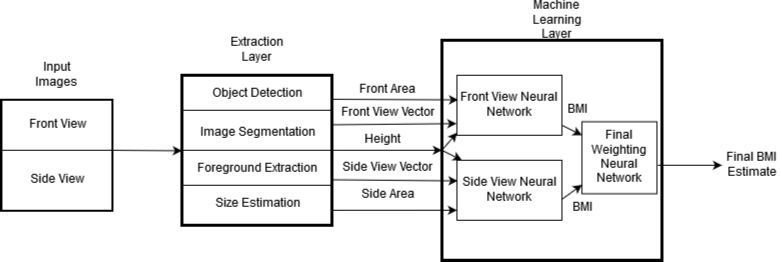
\includegraphics[width=\linewidth]{systemblock.png}
    \caption{System Block Diagram showing the processes input images undergo to estimate BMI.}
    \label{fig:systemblockdiagram}
\end{figure}

\section{Model Estimation Accuracy For Total Dataset}

\begin{figure}[H]
    \centering
    \begin{minipage}[b]{0.35\textwidth}
    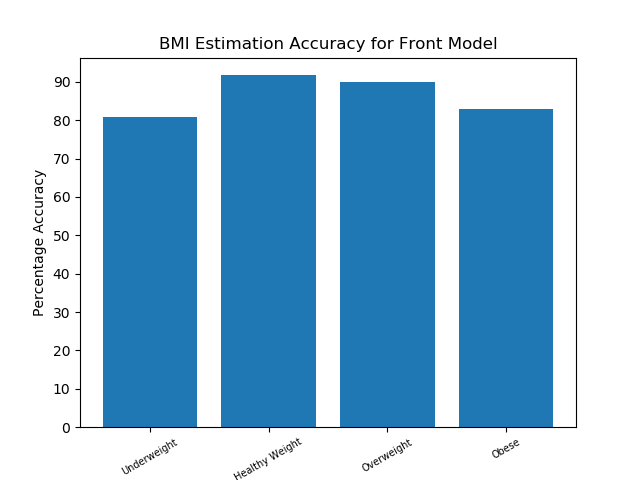
\includegraphics[width=\linewidth]{Front.png}
    \caption{Estimation Accuracy Across BMI Categories for Front Model.}
    \label{fig:frontaccuracy}
    \end{minipage}
    \hspace{1cm}
    \begin{minipage}[b]{0.35\textwidth}
    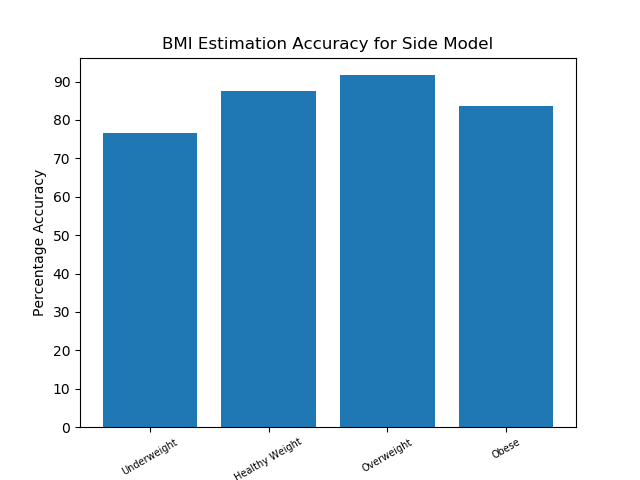
\includegraphics[width=\linewidth]{Side.png}
    \caption{Estimation Accuracy Across BMI Categories for Side Model.}
    \label{fig:sideaccuracy}
    \end{minipage}
\end{figure}

\section{Model Error Distribution For Total Dataset}

\begin{figure}[H]
    \centering
    \begin{minipage}[b]{0.35\textwidth}
    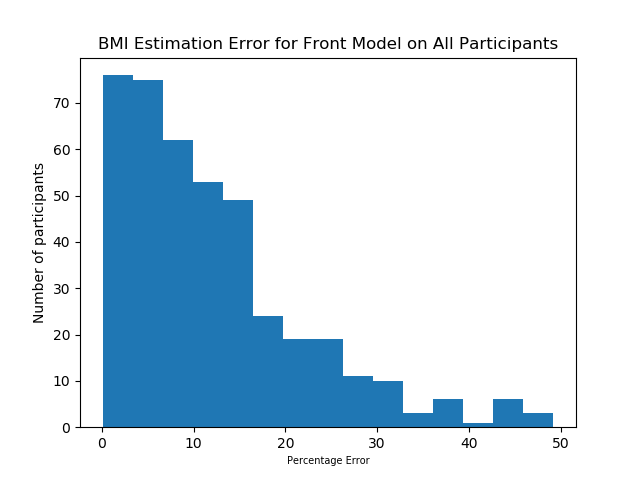
\includegraphics[width=\linewidth]{fronterrorspread.png}
    \caption{Error Distribution Across BMI Categories for Front Model.}
    \label{fig:fronterrorspread}
    \end{minipage}
    \hspace{1cm}
    \begin{minipage}[b]{0.35\textwidth}
    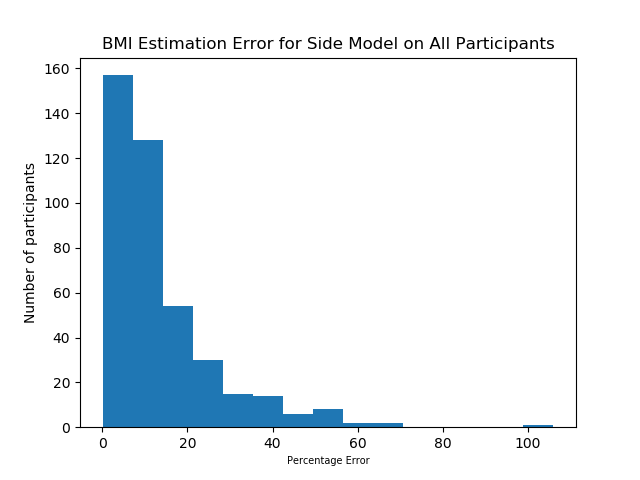
\includegraphics[width=\linewidth]{sideerrorspread.png}
    \caption{Error Distribution Across BMI Categories for Side Model.}
    \label{fig:sideerrorspread}
    \end{minipage}
\end{figure}

\section{Front Model Error Distribution}

\begin{figure}[H]
    \centering
    \begin{minipage}[b]{0.35\textwidth}
    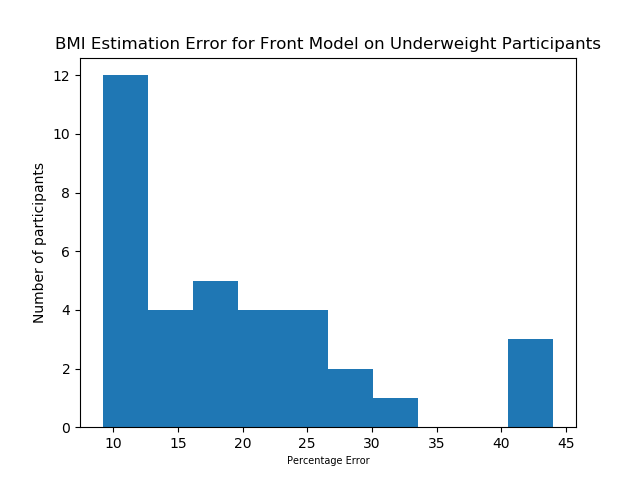
\includegraphics[width=\linewidth]{frontundererror.png}
    \caption{Distribution of Percentage Error for Front Model BMI Estimations performed on the Underweight portion of the dataset.}
    \label{fig:frontundererror}
    \end{minipage}
    \hspace{1cm}
    \begin{minipage}[b]{0.35\textwidth}
    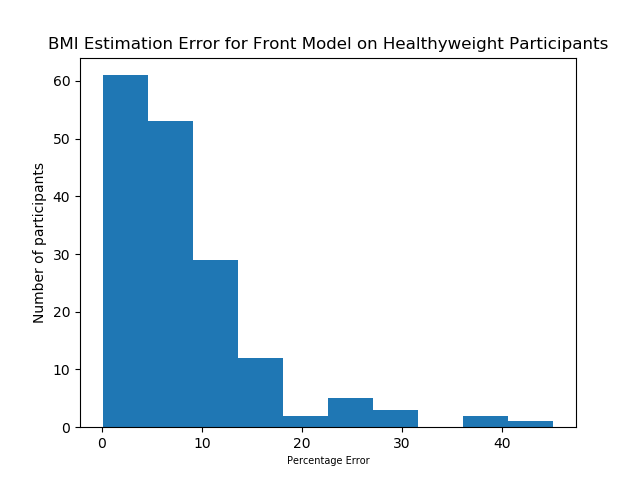
\includegraphics[width=\linewidth]{fronthealthyerror.png}
    \caption{Distribution of Percentage Error for Front Model BMI Estimations performed on the Healthy portion of the dataset.}
    \label{fig:fronthealthyerror}
    \end{minipage}
\end{figure}

\begin{figure}[H]
    \centering
    \begin{minipage}[b]{0.35\textwidth}
    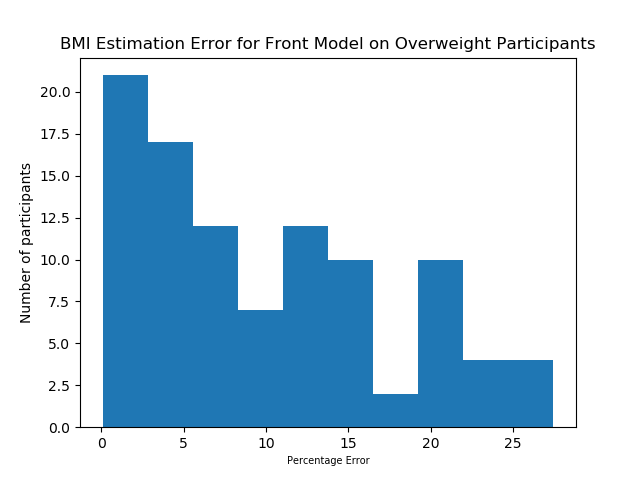
\includegraphics[width=\linewidth]{frontovererror.png}
    \caption{Distribution of Percentage Error for Front Model BMI Estimations performed on the Overweight portion of the dataset.}
    \label{fig:frontovererror}
    \end{minipage}
    \hspace{1cm}
    \begin{minipage}[b]{0.35\textwidth}
    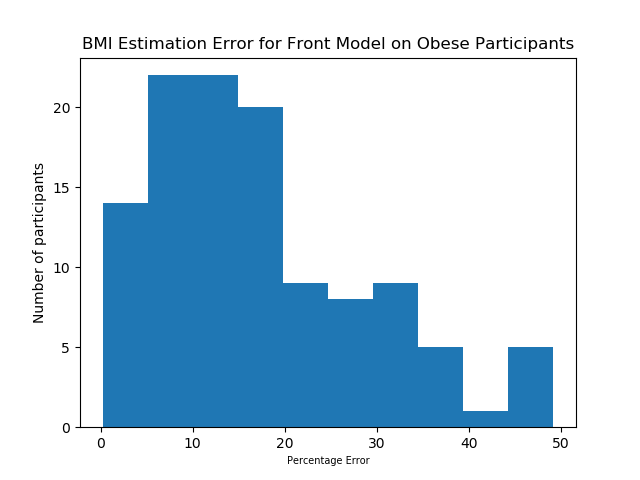
\includegraphics[width=\linewidth]{frontobeseerror.png}
    \caption{Distribution of Percentage Error for Front Model BMI Estimations performed on the Obese portion of the dataset.}
    \label{fig:frontobeseerror}
    \end{minipage}
\end{figure}

\section{Side Model Error Distribution}

\begin{figure}[H]
    \centering
    \begin{minipage}[b]{0.35\textwidth}
    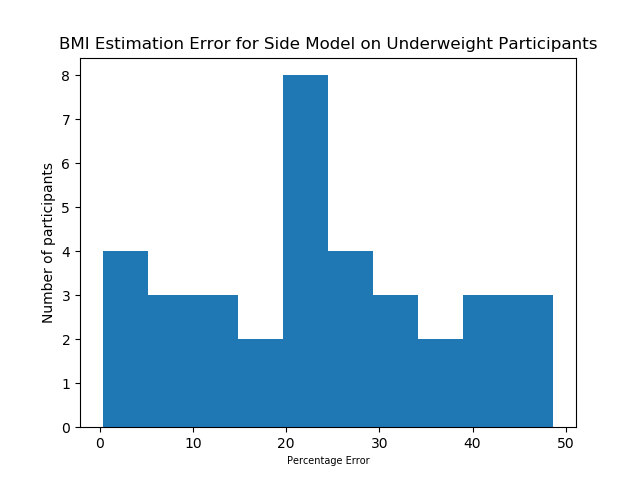
\includegraphics[width=\linewidth]{sideundererror.png}
    \caption{Distribution of Percentage Error for Side Model BMI Estimations performed on the Underweight portion of the dataset.}
    \label{fig:sideundererror}
    \end{minipage}
    \hspace{1cm}
    \begin{minipage}[b]{0.35\textwidth}
    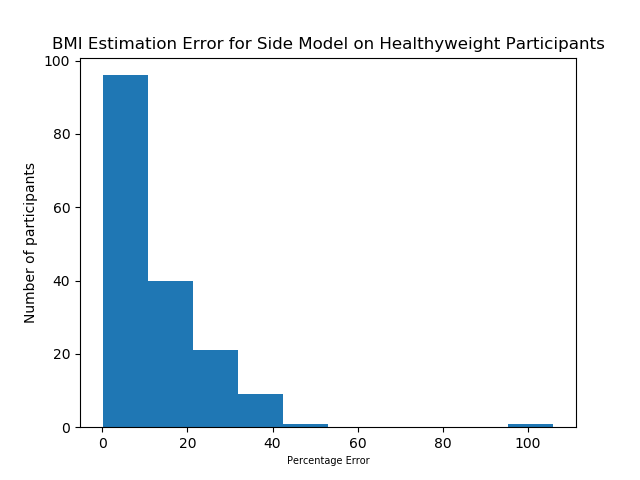
\includegraphics[width=\linewidth]{sidehealthyerror.png}
    \caption{Distribution of Percentage Error for Side Model BMI Estimations performed on the Healthy portion of the dataset.}
    \label{fig:sidehealthyerror}
    \end{minipage}
\end{figure}

\begin{figure}[H]
    \centering
    \begin{minipage}[b]{0.35\textwidth}
    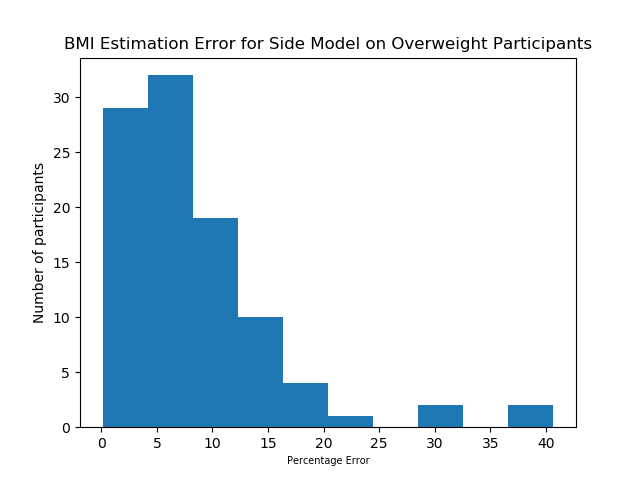
\includegraphics[width=\linewidth]{sideovererror.png}
    \caption{Distribution of Percentage Error for Side Model BMI Estimations performed on the Overweight portion of the dataset.}
    \label{fig:sideovererror}
    \end{minipage}
    \hspace{1cm}
    \begin{minipage}[b]{0.35\textwidth}
    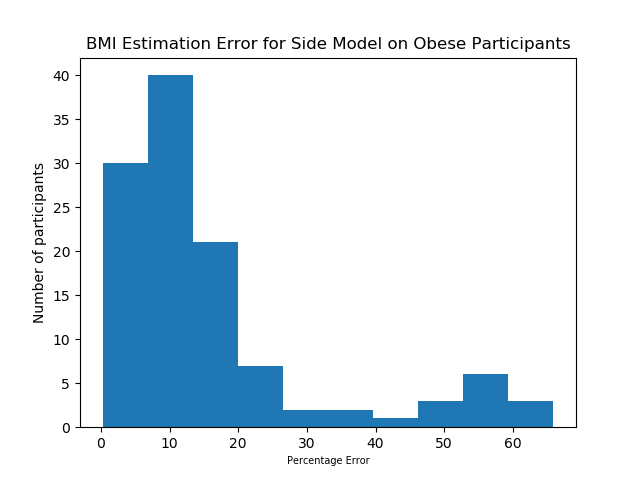
\includegraphics[width=\linewidth]{sideobeseerror.png}
    \caption{Distribution of Percentage Error for Side Model BMI Estimations performed on the Obese portion of the dataset.}
    \label{fig:sideobeseerror}
    \end{minipage}
\end{figure}

\section{Final/Compensator Model Error Distribution}

\begin{figure}[H]
    \centering
    \begin{minipage}[b]{0.35\textwidth}
    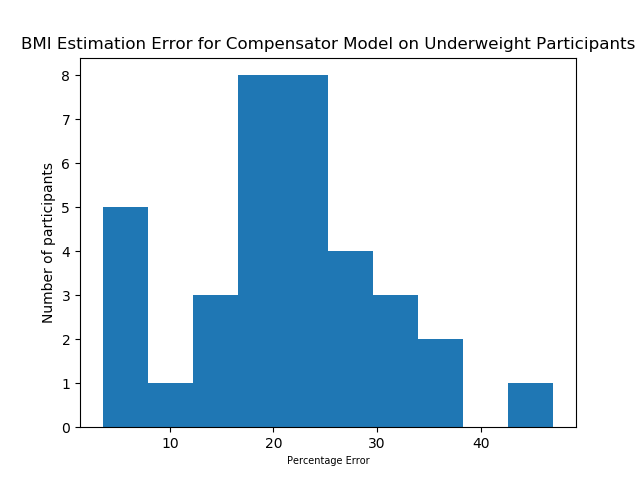
\includegraphics[width=\linewidth]{compundererror.png}
    \caption{Distribution of Percentage Error for Final Model BMI Estimations performed on the Underweight portion of the dataset.}
    \label{fig:compundererror}
    \end{minipage}
    \hspace{1cm}
    \begin{minipage}[b]{0.35\textwidth}
    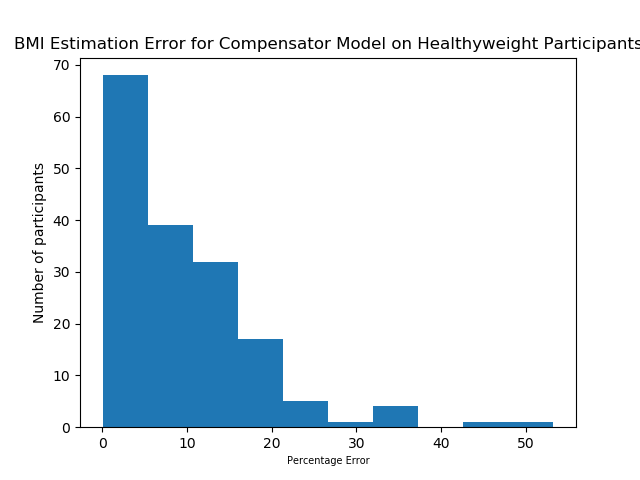
\includegraphics[width=\linewidth]{comphealthyerror.png}
    \caption{Distribution of Percentage Error for Final Model BMI Estimations performed on the Healthy portion of the dataset.}
    \label{fig:comphealthyerror}
    \end{minipage}
\end{figure}

\begin{figure}[H]
    \centering
    \begin{minipage}[b]{0.35\textwidth}
    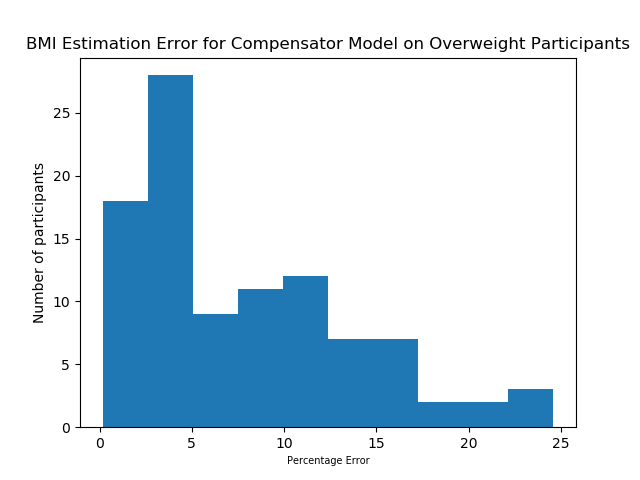
\includegraphics[width=\linewidth]{compovererror.png}
    \caption{Distribution of Percentage Error for Final Model BMI Estimations performed on the Overweight portion of the dataset.}
    \label{fig:compovererror}
    \end{minipage}
    \hspace{1cm}
    \begin{minipage}[b]{0.35\textwidth}
    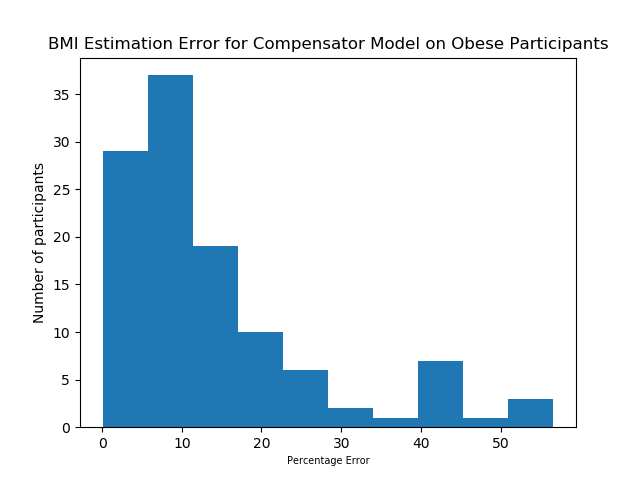
\includegraphics[width=\linewidth]{compobeseerror.png}
    \caption{Distribution of Percentage Error for Final Model BMI Estimations performed on the Obese portion of the dataset.}
    \label{fig:compobeseerror}
    \end{minipage}
\end{figure}

\begin{figure}[H]
    \centering
    \begin{minipage}[b]{0.25\textwidth}
        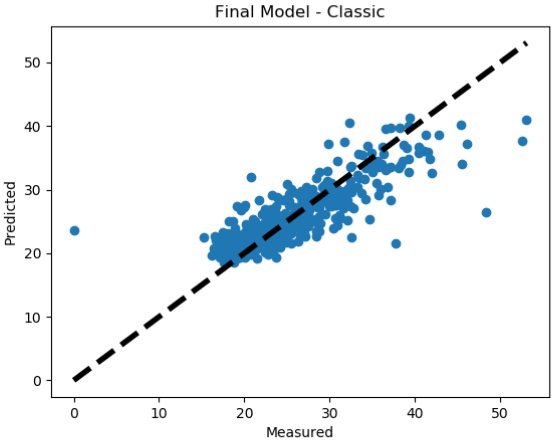
\includegraphics[width=\linewidth]{compscatter.png}
        \caption{Final Model Performance for Total dataset.}
        \label{fig:compscatter}
        \end{minipage}
        \hspace{1cm}
    \begin{minipage}[b]{0.25\textwidth}
    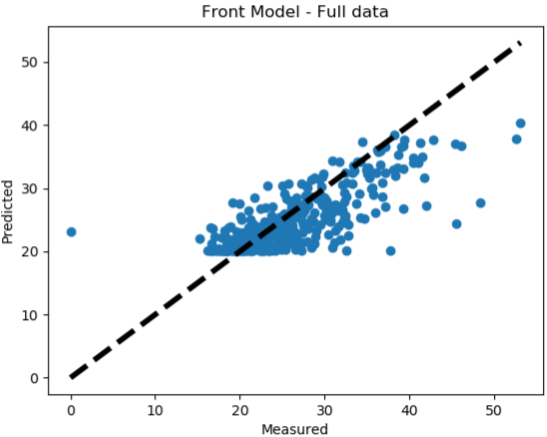
\includegraphics[width=\linewidth]{frontscatter.png}
    \caption{Front Model Performance for Total dataset.}
    \label{fig:frontscatter}
    \end{minipage}
    \hspace{1cm}
    \begin{minipage}[b]{0.25\textwidth}
    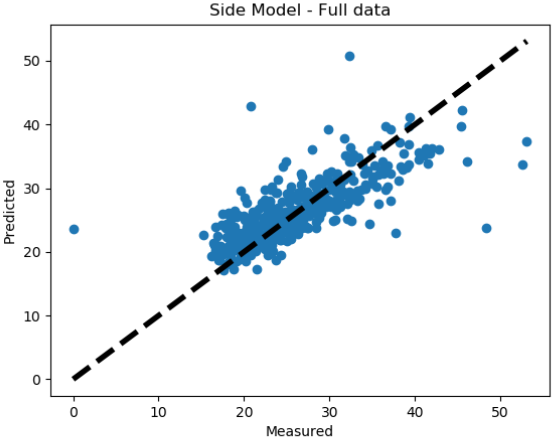
\includegraphics[width=\linewidth]{sidescatter.png}
    \caption{Side Model Performance for Total dataset.}
    \label{fig:sidescatter}
    \end{minipage}
\end{figure}
\end{document}

% budget
% system diagrams